\expandafter\ifx\csname ifdraft\endcsname\relax
 \begin{document}
\fi

\section{検証}

計算の章(\ref{sec:calculation})で述べたように,多くの各種計算値は酸素摂取量VO_2を元に算出される.そこで,今回は実験により運動中の酸素摂取量を測定することによって装置の検証を行う.

酸素摂取量の測定には,トレッドミルや自転車エルゴメーター,踏み台などが用いられる.今回は自宅で実験を行うため,パワーメーター(出力計)を装着したロードバイクを自動負荷調整機能付きのローラー台に取り付けて検証を行った(図\ref{fig:bike_in_use}).
自転車エルゴメーターを使用した酸素摂取量の測定の慣例に従いケイデンス(ペダル回転数)を60rpmに固定した上で,酸素摂取量パワー(出力)をもとに負荷を指定したワークアウトを実行する.ケイデンスを60rpmに固定しているので,パワー(W)を60で割った値が負荷(kp)となる.
ワークアウト中の酸素摂取量に加えて,ロードバイクや身体に取り付けたセンサーによってパワー(W),心拍数(bpm),ケイデンス(rpm)などを測定し,それらの値と酸素摂取量を比較することで装置の有用性について検証する.

\begin{figure}[H]
  \begin{center}
    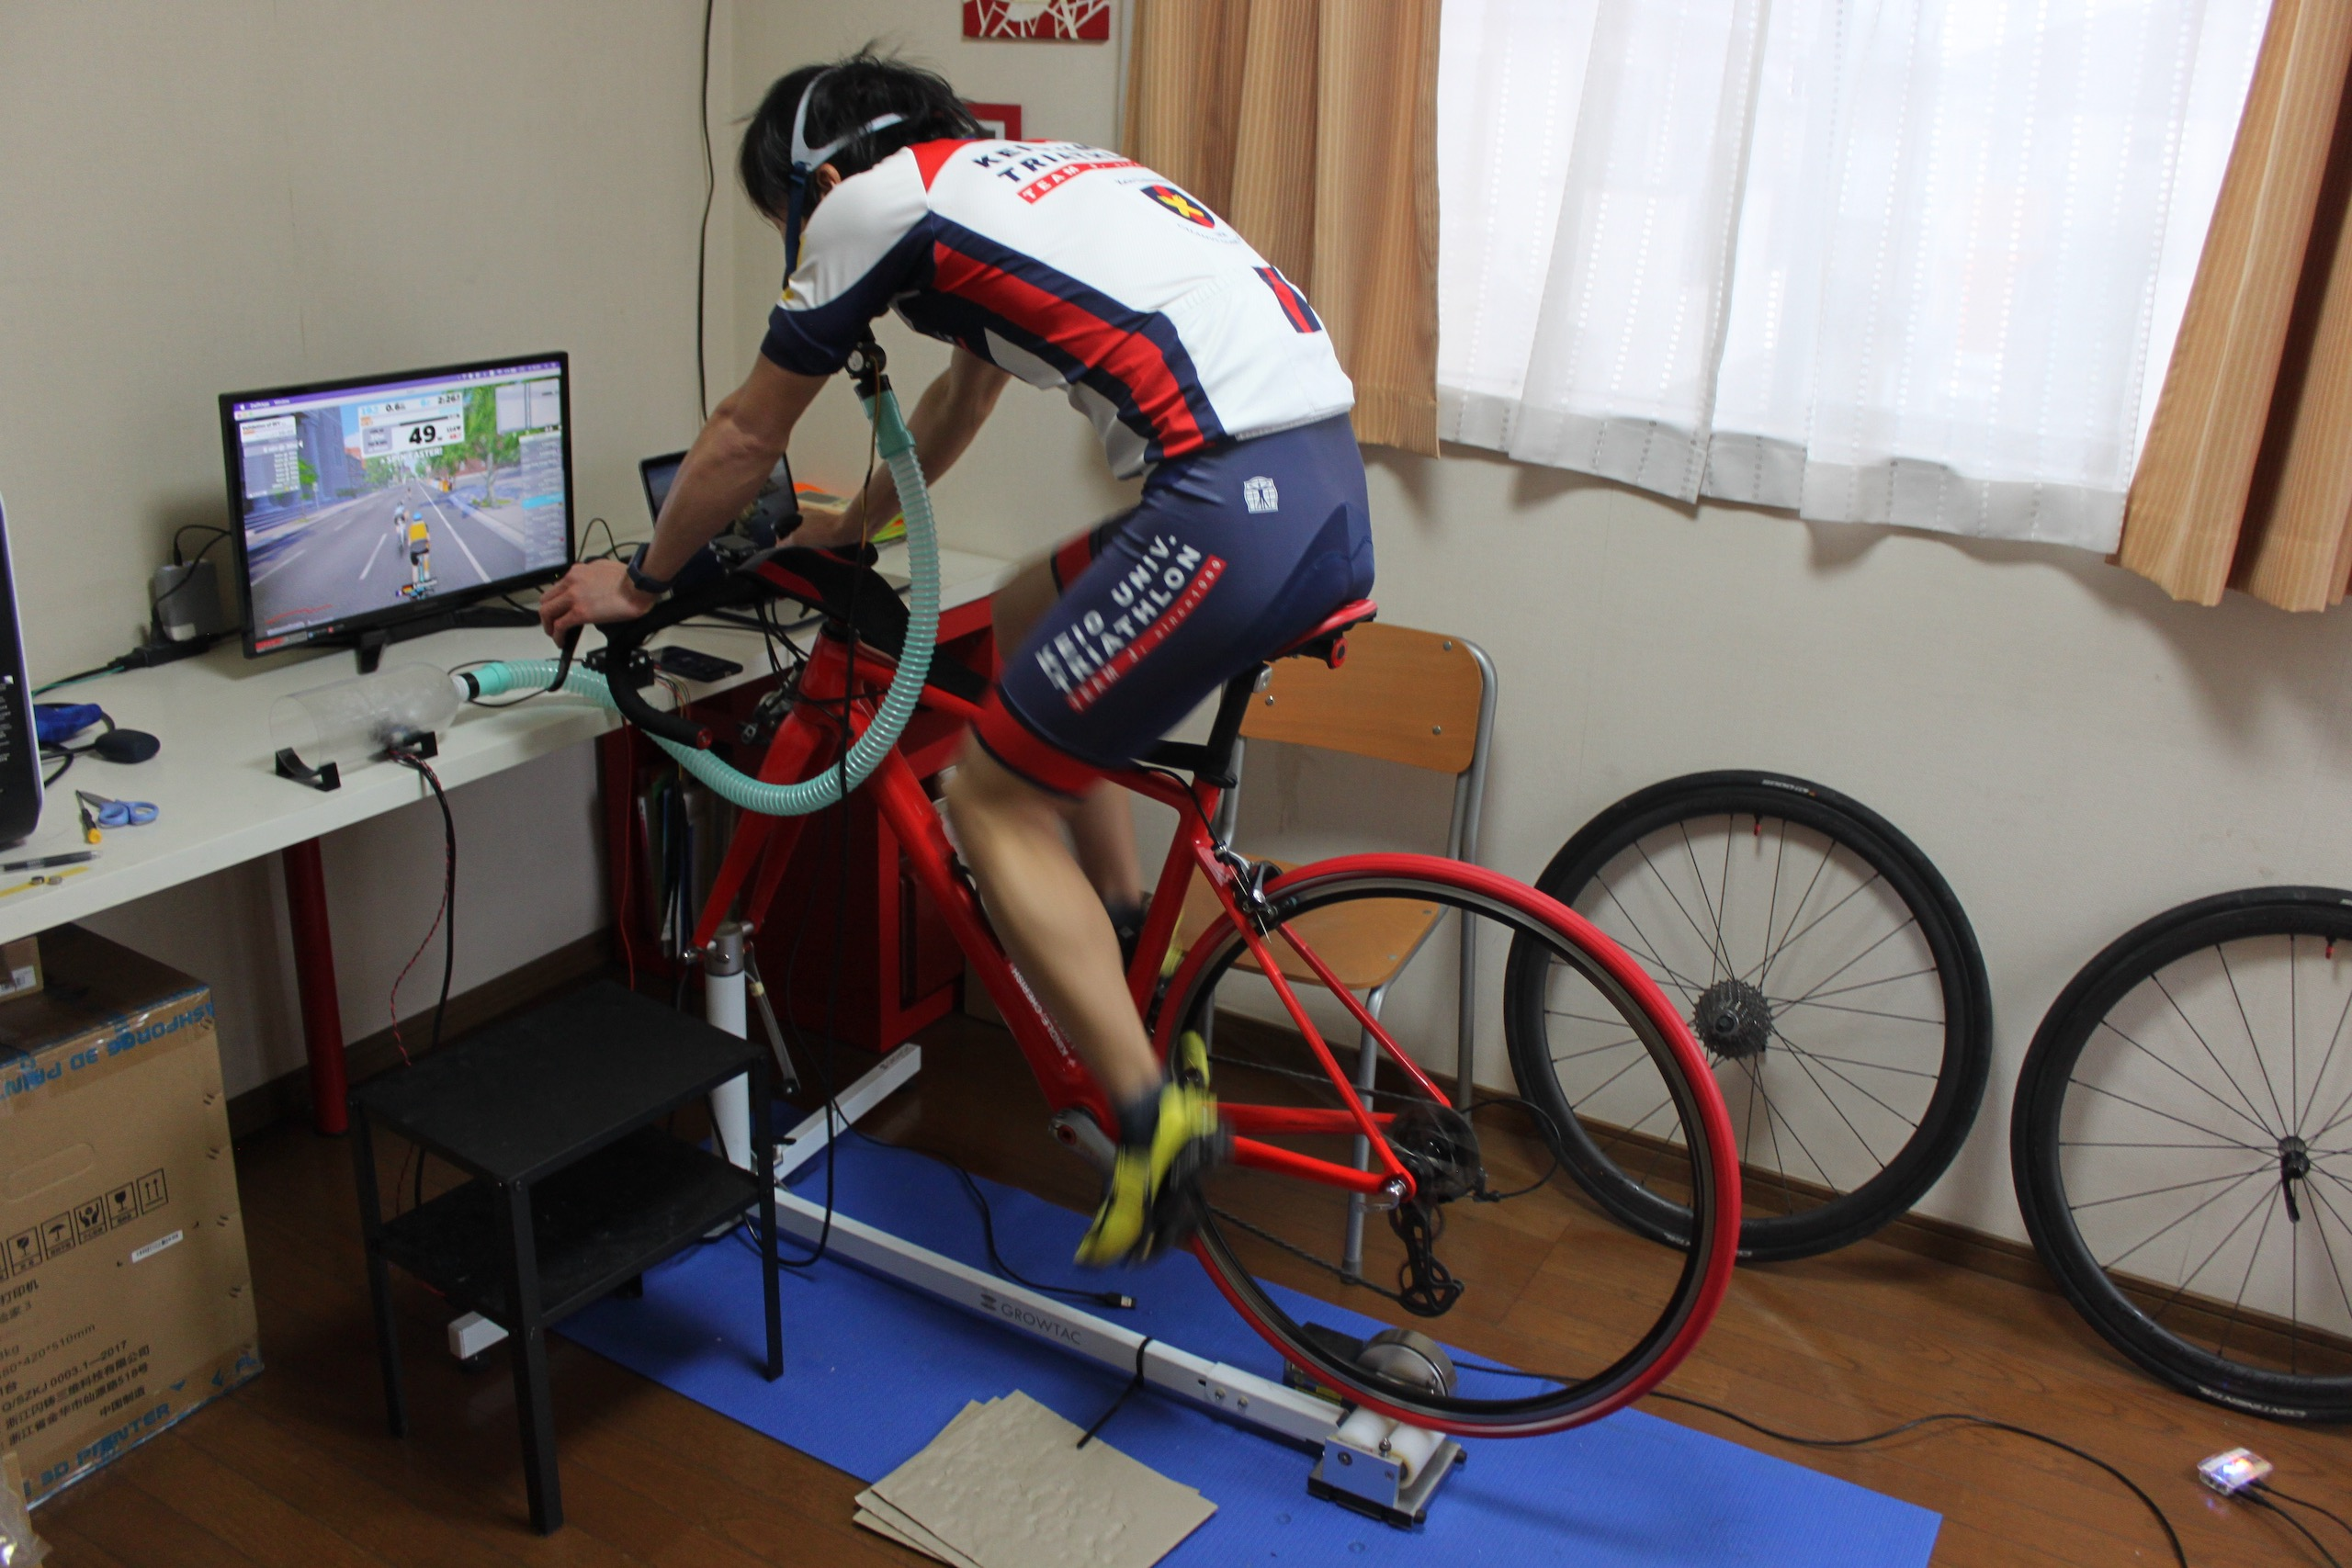
\includegraphics[width=10cm]{fig/bike_in_use}
    \caption{実験の様子}
    \label{fig:bike_in_use}
  \end{center}
\end{figure}

なお,今回の検証は新型コロナウィルス感染症緊急事態宣言中に行った.呼吸代謝測定装置はマスク部などに唾液が多く付着するため,感染防止の観点から複数人の被験者を対象にした実験を行うことが難しい.よって,実験は筆者が自宅にて自身一人を被験者として行っている.ご了承いただきたい.

%様々な点で装置の検証を行うため,以下の3つの実験を行った.

%\begin{enumerate}
  %\item ランプアップ・ダウン
  %\item 最大酸素摂取量測定
  %\item 負荷変動を伴うワークアウト
%\end{enumerate}

%以上の実験を行った上で,装置が出力するログデータとその他のセンサーで測定したデータをタイムスタンプを用いて統合して検証を行う.

\subsection{実験方法}

最大酸素摂取量(\.{V}O_2Max)以下の低強度で自転車を漕ぐ時,パワーが高いほど酸素摂取量が多くなるはずである.これが実験により確認できるかを検証する.漸増負荷法の定常状態ありの連続負荷法のプロトコルに従い\cite{science_of_vo2},3分ごとに負荷を漸増するという実験を,低強度プロトコルと高強度プロトコル,2種類の設定パワーで行う.それぞれで酸素摂取量を測定し,酸素摂取量とパワー,心拍数を比較することで装置の有効性を検証する.

\subsubsection{実験プロトコル}

酸素摂取量が最大酸素摂取量に近付く高強度の運動では,無酸素系の酸素共有量の不足分(酸素借)を運動を止めた後も有酸素系が補い続けるために安静時よりも酸素摂取量が高い状態が続く.これを酸素負債と呼ぶ.実験に使用する設定パワーは,有酸素系の酸素摂取量のみを見るために,酸素負債が発生しないように出来る限り低強度に設定する.

予備実験から,機材の都合上,ケイデンス60rpmを保ったまま出力できる最低パワーは40W付近であることが分かった.そこで,低強度プロトコルにおける第1段階パワーを40Wとし,高強度プロトコルにおいては30W(ケイデンス60rpm時において0.5kp)増負荷として70Wとした.第1段階パワーからそれぞれ3oW刻みで3分ごとに増負荷とし,設定パワーは表\ref{tb:protocol_power}のようになる.

\begin{table}[]
\begin{center}
  \caption{各プロトコルの設定パワー}
  \label{tb:protocol_power}
  \begin{tabular}{|l|l|l|}
  \hline
       & 低強度プロトコル & 高強度プロトコル \\ \hline
  第1段階 & 40W      & 70W      \\ \hline
  第2段階 & 70W      & 110W     \\ \hline
  第3段階 & 110W     & 140W     \\ \hline
  第4段階 & 140W     & 170W     \\ \hline
  \end{tabular}
\end{center}
\end{table}

本研究で製作した装置は各値の算出に1分平均値を使用しているため,平均値が立ち上がるまでの測定開始後1分間のデータは除外する必要がある.そのため第一段階パワーに入るまでに,40Wでのペダリングをウォーミングアップを兼ねて5分間行い,実際のデータ処理では測定開始後2分後からのデータを用いることとした..以上より,低強度プロトコル,高強度プロトコルはそれぞれ図\ref{fig:protocol_rampup_light},図\ref{fig:protocol_rampup_hard}のようになる.

\begin{figure}[h]
  \begin{center}
    \label{fig:protocol_rampup_light}
    \caption{低強度プロトコル}
    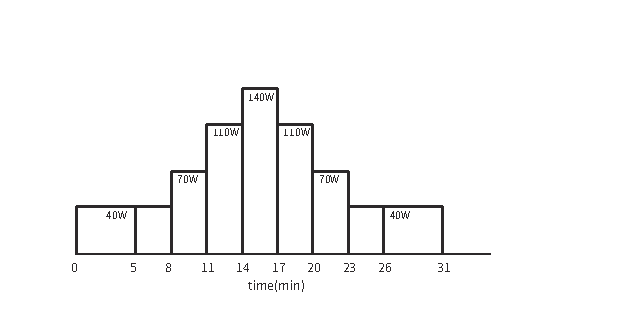
\includegraphics[width=12cm]{fig/protocol_rampup_light.pdf}
  \end{center}
\end{figure}

\begin{figure}[h]
  \begin{center}
    \label{fig:protocol_rampup_hard}
    \caption{高強度プロトコル}
    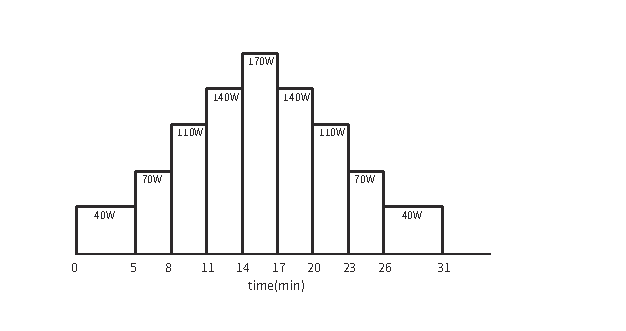
\includegraphics[width=12cm]{fig/protocol_rampup_hard.pdf}
  \end{center}
\end{figure}

\subsection{実験機材}

作成したプロトコルを元に運動を行うためにZwiftのワークアウト機能を用いた.Zwiftはパワーメーター等のパワーソースを接続し,入力されたパワーを元にバーチャルワールド内を自転車に乗ったアバターを操作して走ることができるバーチャルサイクリングプラットフォームである(図\ref{fig:zwift}).Zwiftはパワーや心拍数,ケイデンスなどの走行ログデータが1秒間隔で記録されたFITファイルを保存する.これをmacOS用のユーティリティー,FIT FIle Explorer\cite{fitfile}を用いてCSVファイルに変換した.

\begin{figure}[h]
  \begin{center}
    \label{fig:zwift}
    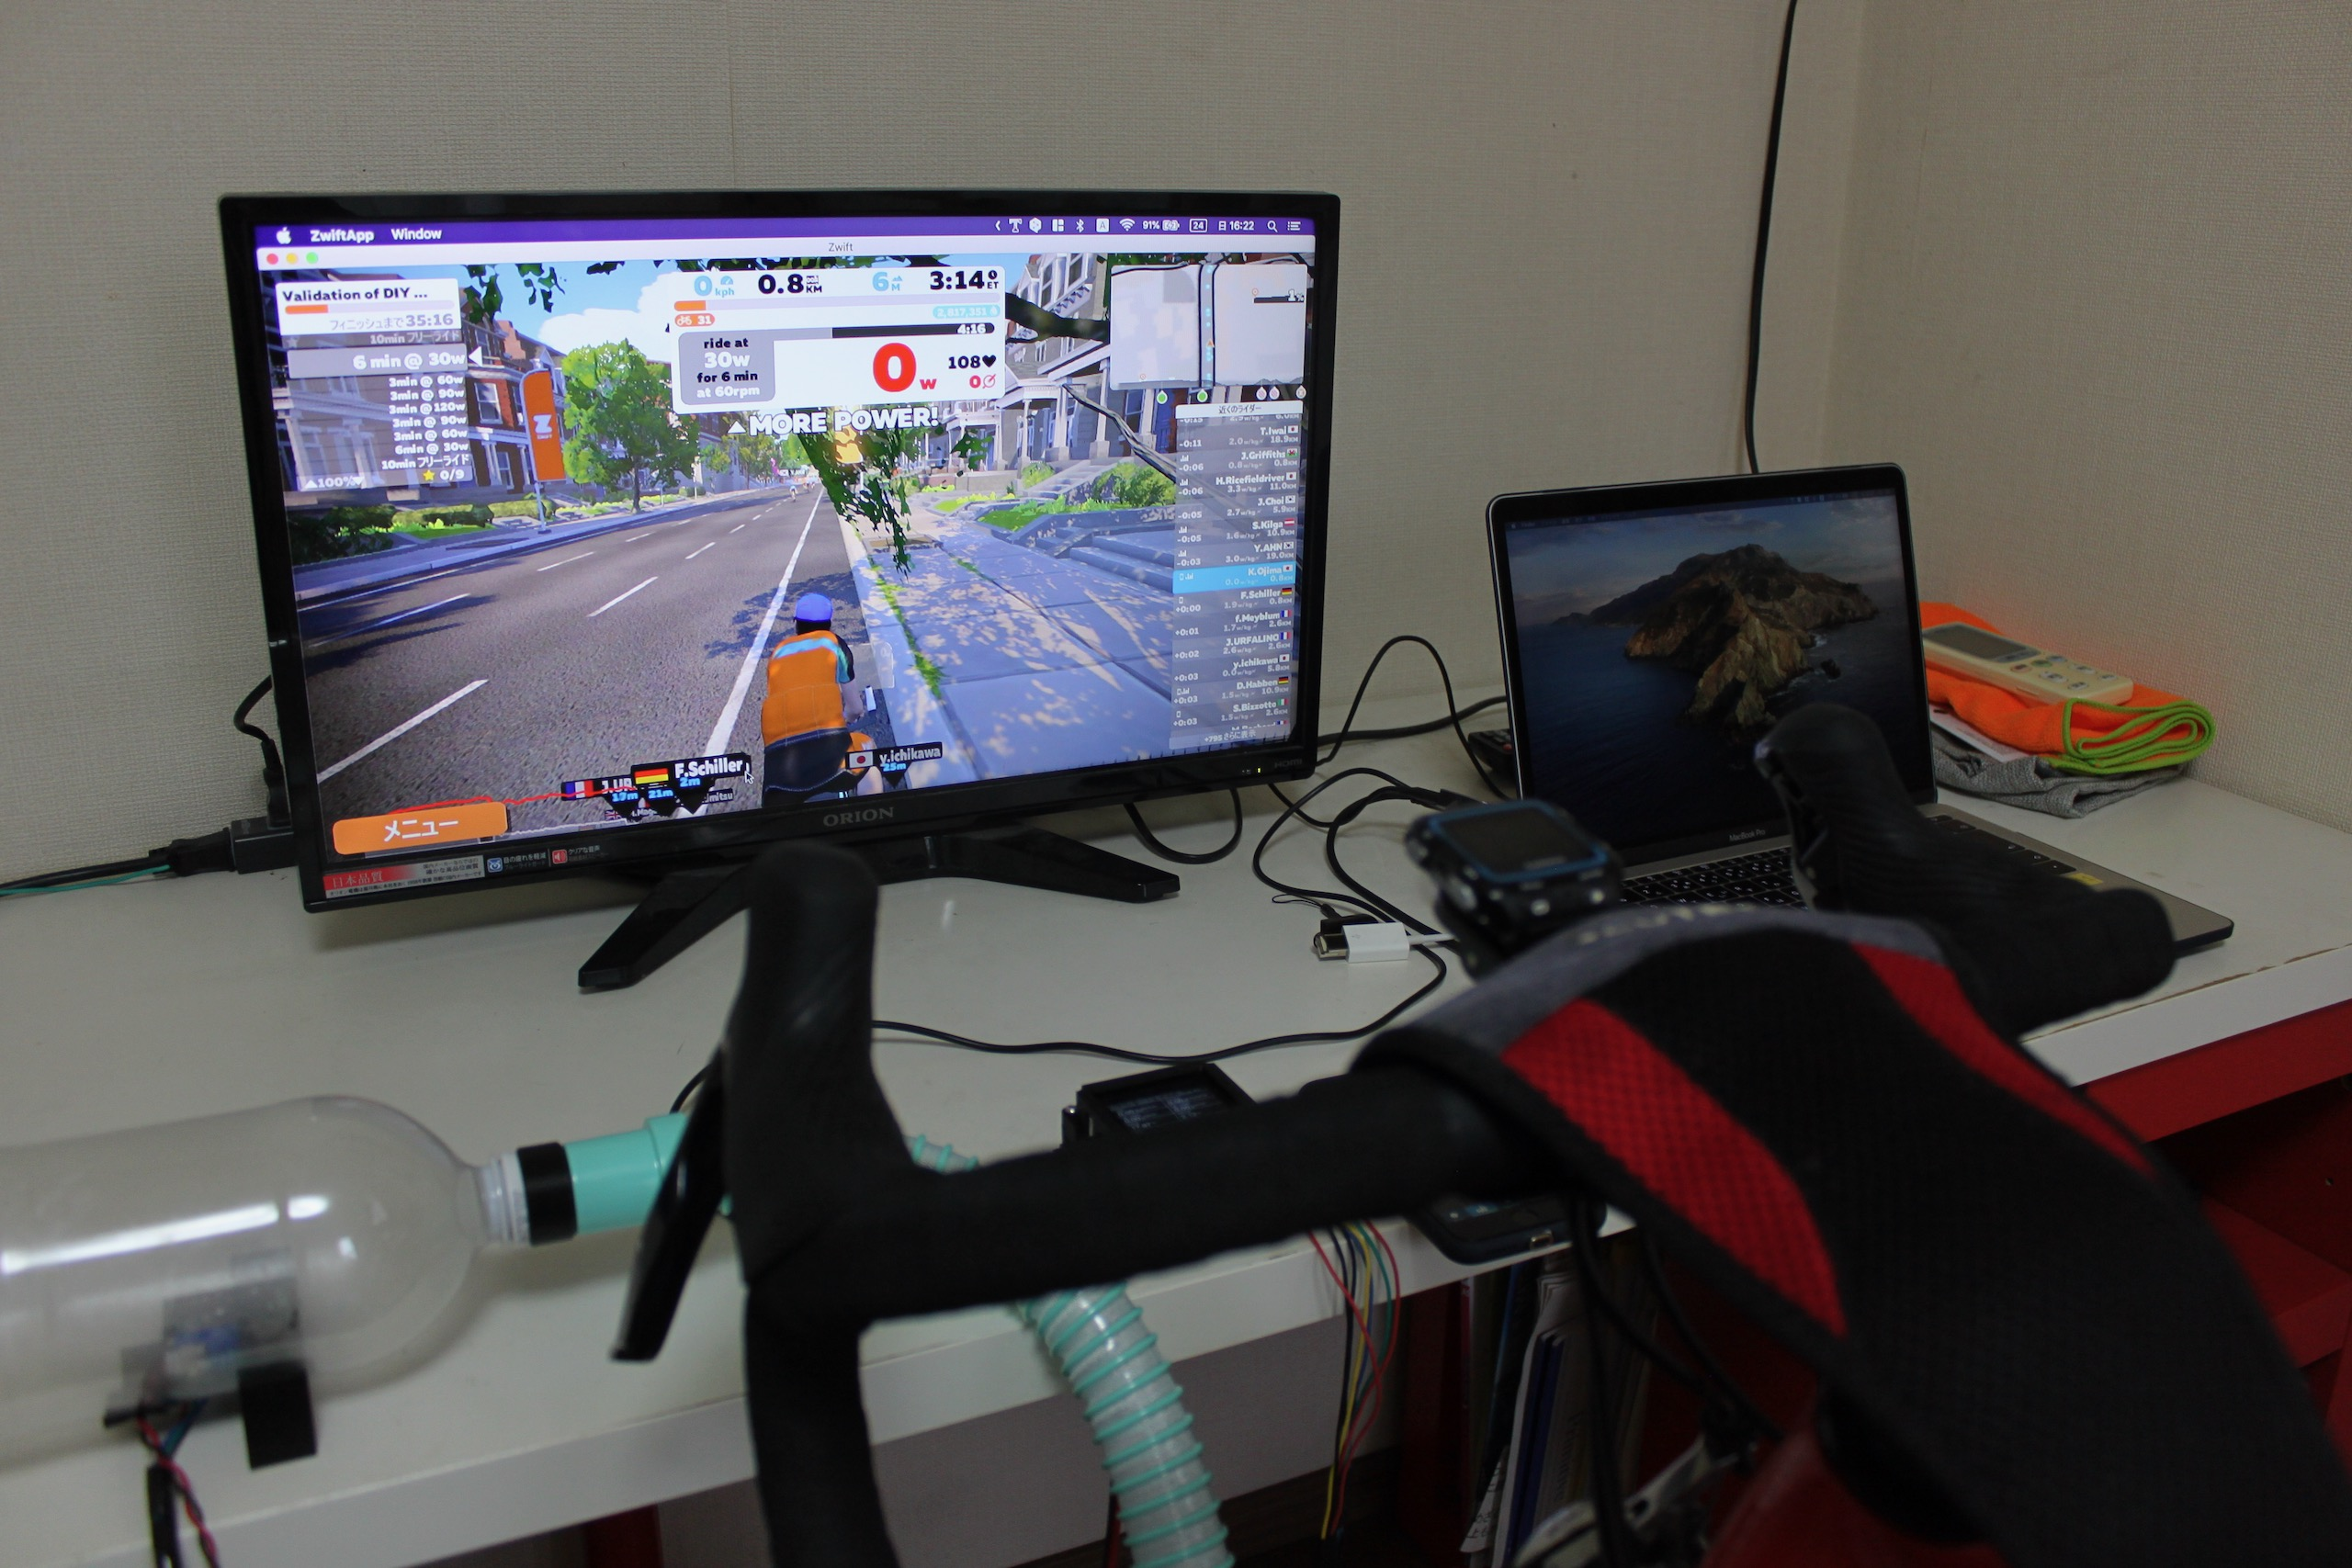
\includegraphics[width=8cm]{fig/zwift}
    \caption{Zwiftの実行環境}
  \end{center}
\end{figure}

Zwiftのワークアウト機能はペダリングを開始した時点を0秒とし,その時刻からログデータファイルの記録を開始する.今回製作した装置は1秒間隔でログデータを記録しタイムスタンプを付与する.Zwiftが出力するログデータの記録開始時刻から2分後の時刻を基準とし,両ログデータの同期を行った.

今回使用したパワーメーターは,4iiii InnovationsのPrecision 2.0 3D(図\ref{fig:4iiii})である.自転車運動のパワーを測定する方法は複数あるが,このパワーメーターは左側のクランクアームの裏側に貼り付けた歪みゲージによって計測されたトルクと,加速度センサーによって計測されたケイデンス(ペダル回転数)からパワーを算出する一般的なタイプである.ZwiftとはANT+方式で接続した.

Zwiftが出力するログデータにはPrecision 2.0 3Dが出力する1秒パワーが1秒間隔で記録される.これは変動が大きく, 1分間平均値となる酸素摂取量と比較するのは困難であったため,後処理によって1分平均パワー値を計算して使用した.

\begin{figure}[h]
  \begin{center}
    \label{fig:4iiii}
    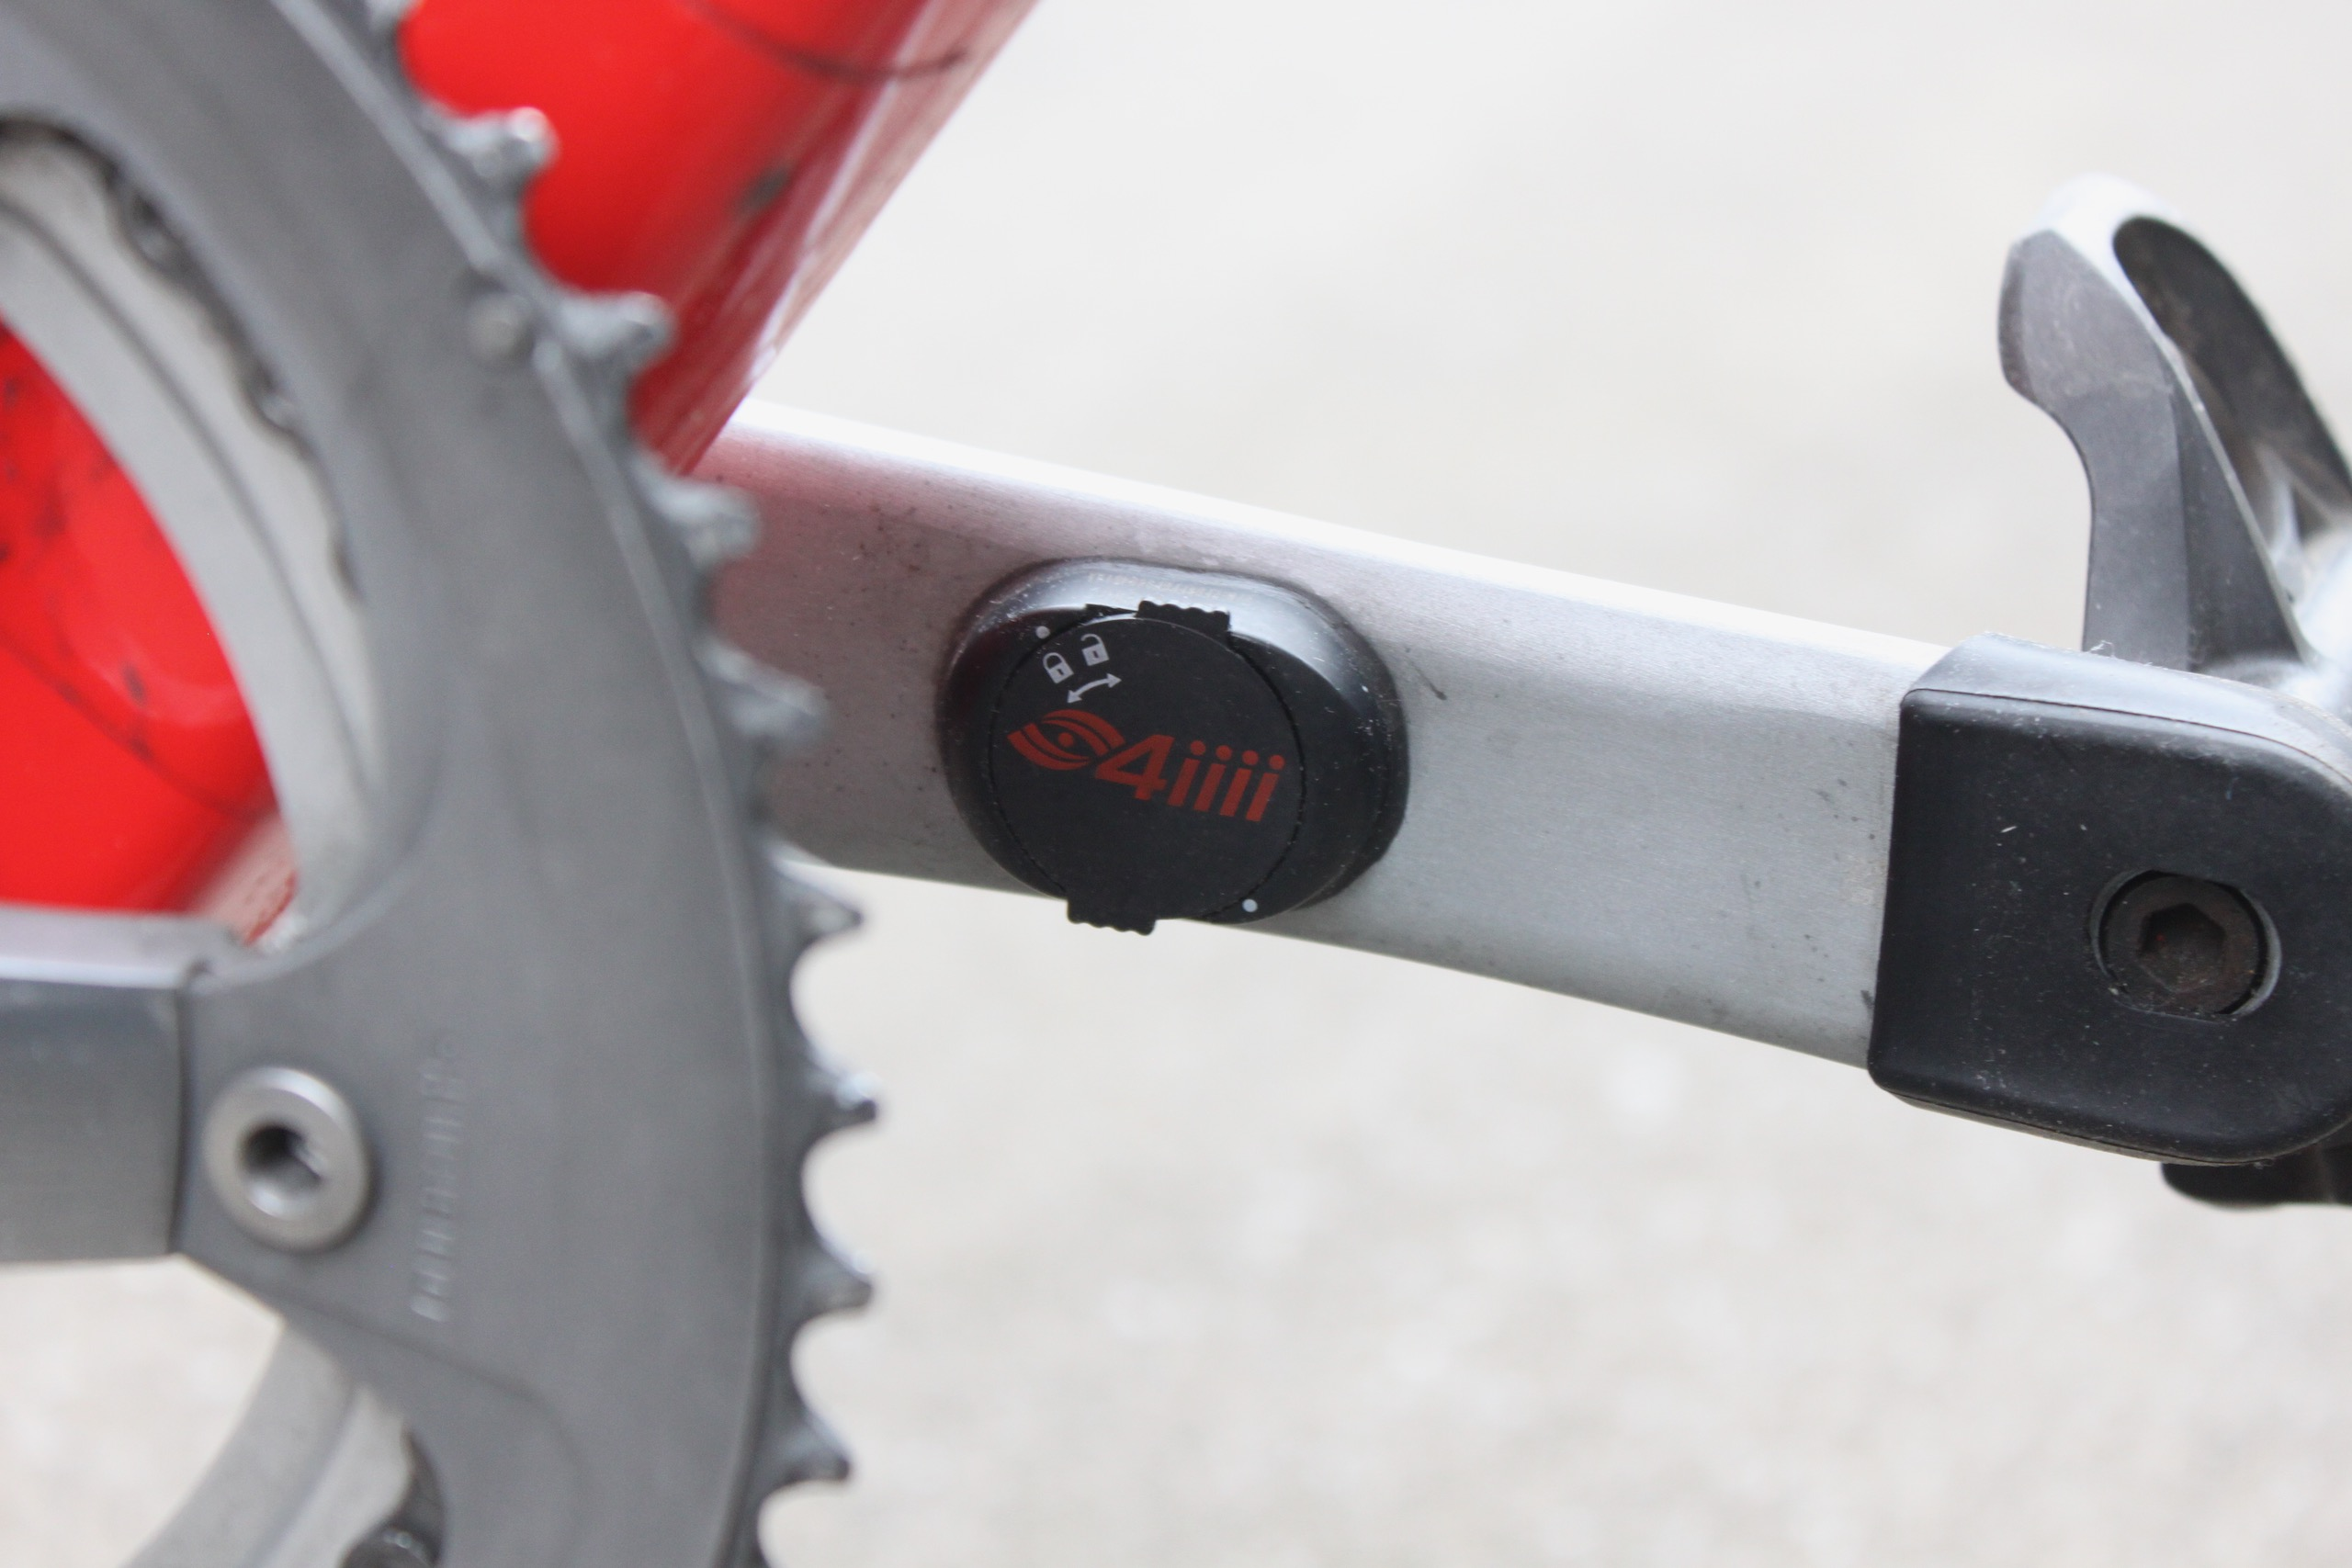
\includegraphics[width=8cm]{fig/4iiii}
    \caption{4iiii Innovations Precision 2.0 3D}
  \end{center}
\end{figure}

自動負荷調整機能付きローラー台にはGROWTACのハイブリッド式(前輪固定式)ローラー台のGT-ROLLER Flex3(図\ref{fig:gt-roller_flex3})を用いた.なお,自動負荷調整装置であるGT-ePower-FとGT-eBoxを取り付けているが,今回の実験においては自動負荷調整機能は無効化し最低負荷に固定して使用している.

\begin{figure}[h]
  \begin{center}
    \label{fig:gt-roller_flex3}
    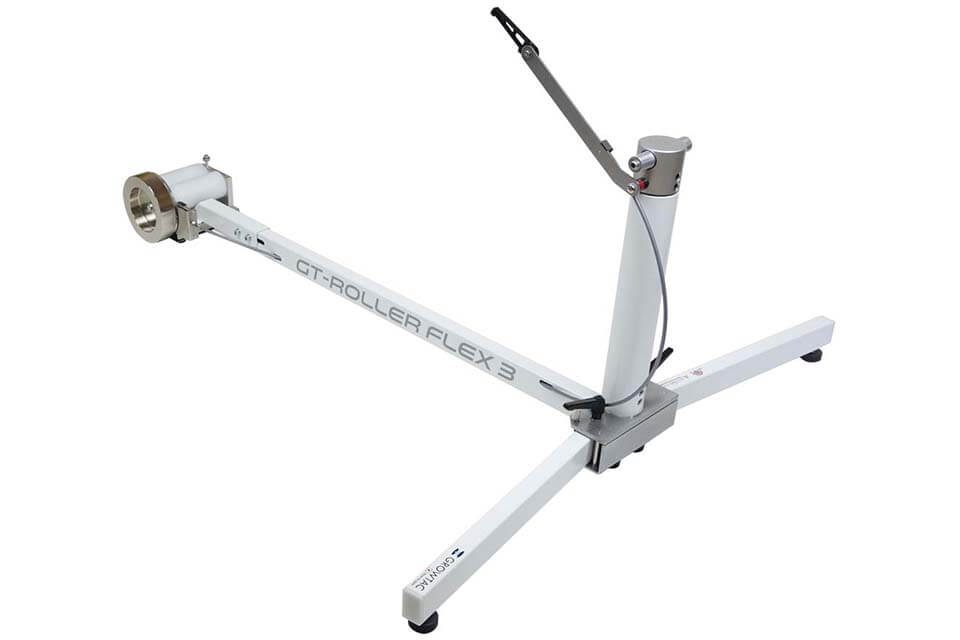
\includegraphics[width=8cm]{fig/gt-roller_flex3}
    \caption{GT-Roller Flex3(写真は手動負荷調整装置付き)}
  \end{center}
\end{figure}

心拍数の測定にはScoscheの光学式心拍計のRHYTHM+を使用した.光学式心拍計は皮膚に光を照射し,血管内の反射を読み取ることで脈拍を計測する.この心拍計は光源に3つのLED(緑色2個,黄色1個)を使用している.本来は前腕内側に巻きつけることが推奨されているが,皮下脂肪量が多い上腕外側に巻きつけて使用した方が異常値の出力の頻度が低くなることが確認できているため,上腕外側に巻きつけて心拍数を計測した.ZwiftにはANT+方式で接続した.

\begin{figure}[h]
  \begin{center}
    \label{fig:rhythm}
    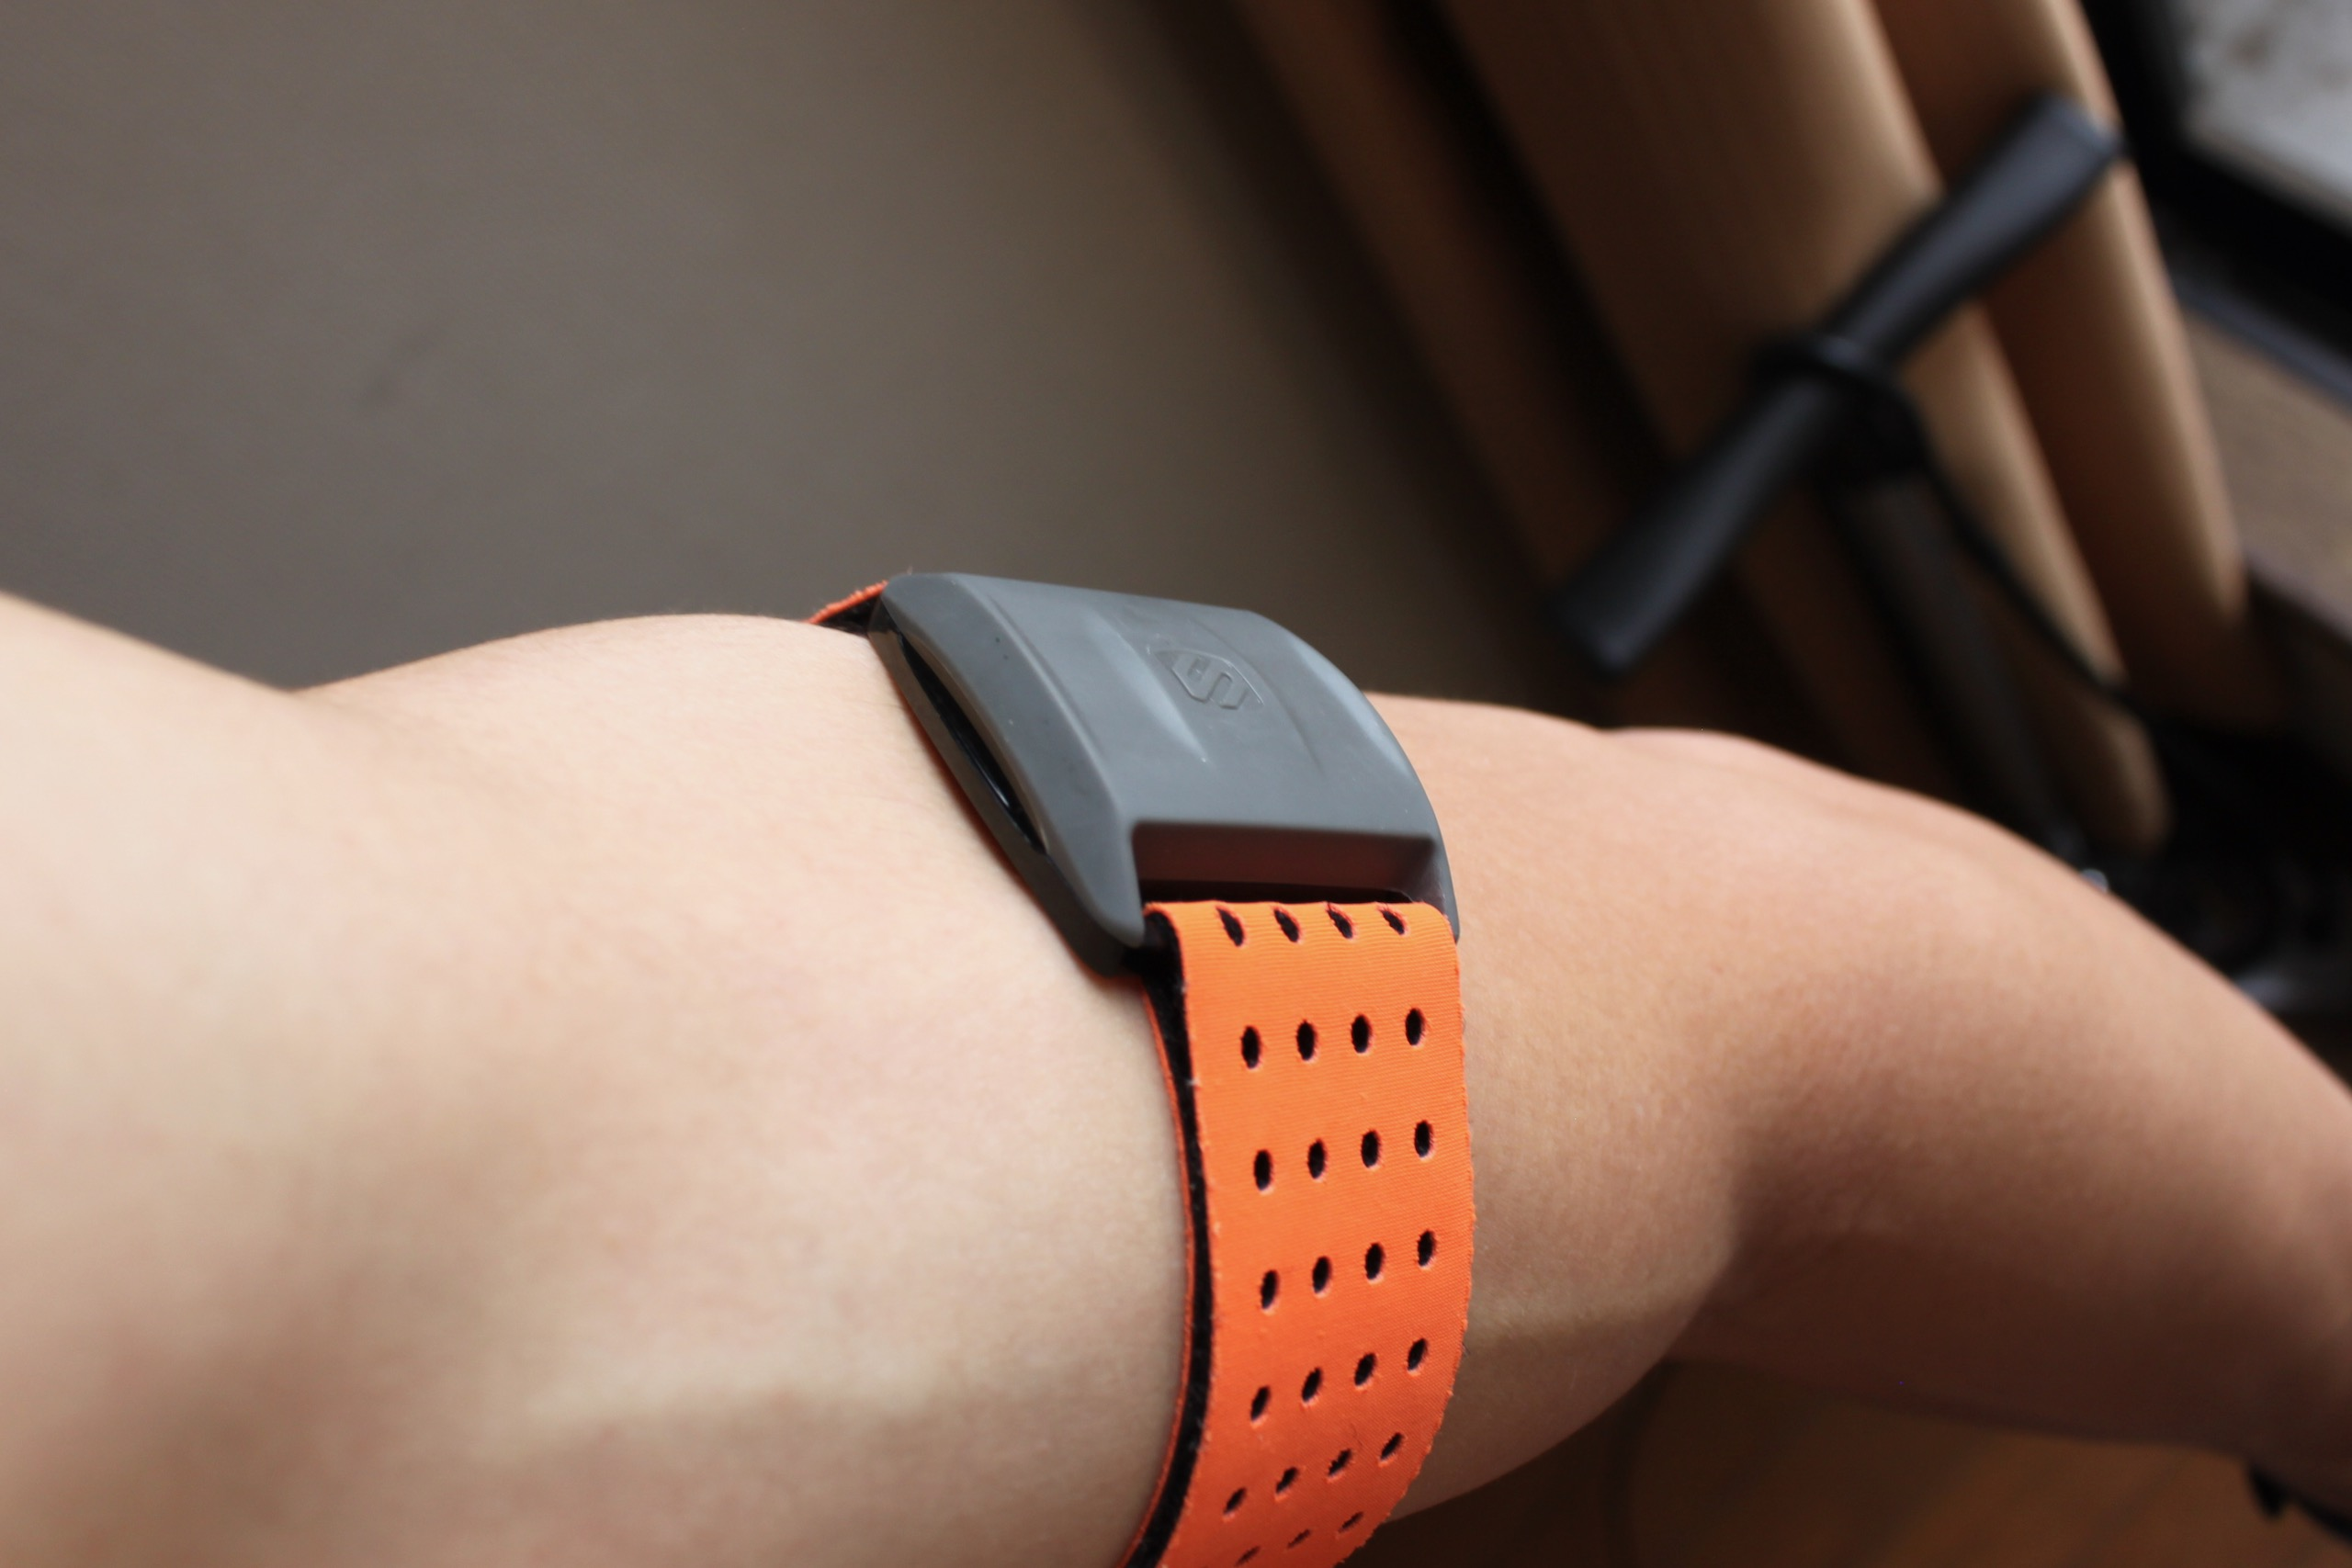
\includegraphics[width=8cm]{fig/rhythm}
    \caption{RHYTHM+(今回は上腕外側に巻きつけて使用)}
  \end{center}
\end{figure}

\subsection{実験条件}

実験は各プロトコル別日に行った.以下に実験時の条件を示す.

\begin{table}[h]
  \begin{center}
  \caption{ランプアップ・ダウン(低強度)}
  \label{tb:YFS201_specsheet}
    \begin{tabular}{ll}
      実験日 & 2021/01/24 \\
      開始時刻 & 10:30:46 \\
      体重 & 55.0kg \\
      気温(平均) & 12mm \\
      大気圧(平均) & 1-30L/min \\
      飽和水蒸気圧(平均) & 1L_{水} = 450pulse \\
      STPD係数(平均) & 1L_{水} = 450pulse
    \end{tabular}
  \end{center}
\end{table}

\begin{table}[h]
  \begin{center}
  \caption{ランプアップ・ダウン(高強度)}
  \label{tb:YFS201_specsheet}
    \begin{tabular}{ll}
      実験日 & 2021/01/25 \\
      開始時刻 & 9mm \\
      体重 & 55.0kg \\
      気温(平均) & 12mm \\
      大気圧(平均) & 1-30L/min \\
      飽和水蒸気圧(平均) & 1L_{水} = 450pulse \\
      STPD係数(平均) & 1L_{水} = 450pulse
    \end{tabular}
  \end{center}
\end{table}

\expandafter\ifx\csname ifdraft\endcsname\relax
  \end{document}
\fi
